\documentclass[10pt]{article}
\usepackage[utf8]{inputenc}
\usepackage[english]{babel}
\usepackage{graphicx}
\usepackage{amsmath}
\usepackage{amssymb}
\usepackage{hyperref}
\usepackage{tikz}

\newcommand{\dd}{\mathrm{d}}

\renewcommand{\vec}[1]{\mathbf{#1}}
\newcommand{\ve}{\vec{e}}
\newcommand{\vi}{\vec{i}}
\newcommand{\vn}{\vec{n}}
\newcommand{\vx}{\vec{x}}

\begin{document}

\title{Memristor mathematical model, ver. 1.0}
\author{https://github.com/eugnsp/memristor}
\maketitle
\tableofcontents

% ================================================================================
\section{Introduction}

This is a succinct formal description of equations, their discretization and
algorithms used for memristor modelling. Gauss units are used in equations and
atomic units are used in the code.

We assume the system to be cylindrically symmetric. 2D finite element schemes
are employed for the Poisson and the heat equations. A 3D grid is used for
the Monte-Carlo simulation of O-vacancies motion with subsequent averaging
over the polar angle.

The geometry of the system is shown in fig.~\ref{fig:system_geometry}. The
geometry is defined in an external mesh file. Numerical physical tags in the mesh
file are used to discern different regions.

\begin{figure}[!ht]
	\centering
	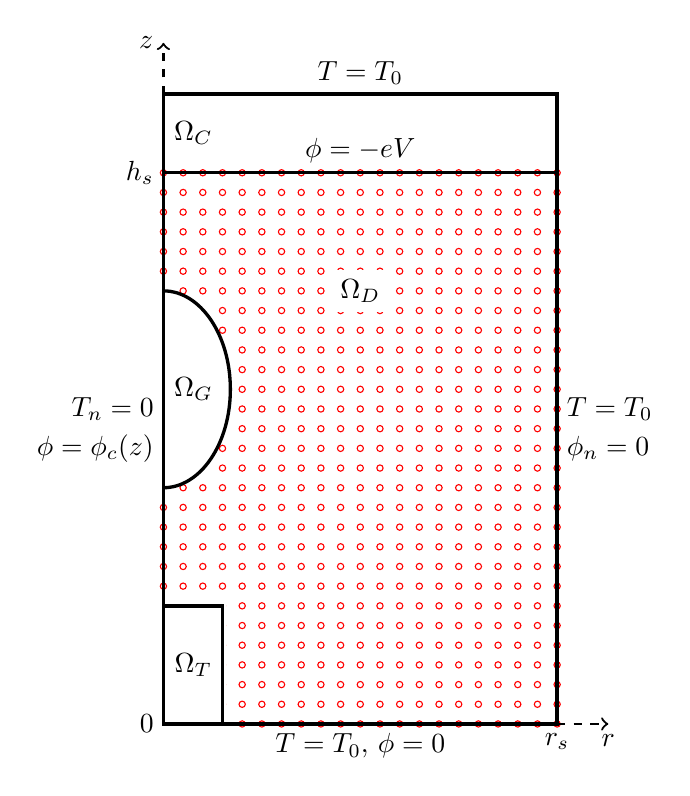
\begin{tikzpicture}
		\foreach \x in {0, .25, ..., 5}	\foreach \y in {0, .25, ..., 7}
		\draw[red] (\x, \y) circle (.04);

		\path[fill=white] (-.1, -.1) -- ++(.9, 0) -- ++(0, 1.7) -- ++(-.9, 0);
		\path[fill=white] (-.1, 2.9) -- ++(.2, 0) -- ++(0, .2) -- ++(.5, 0) --
			++(0, .5) -- ++(.3, 0) -- ++ (0, 1.3) -- ++(-.3, 0) -- ++(0, .5) --
			++(-.45, 0) -- ++(0, .2) -- ++(-.3, 0);

		\draw (.38, 4.25) node[fill=white] {$\Omega_G$};
		\draw (.38, .75) node {$\Omega_T$};
		\draw (.38, 7.5) node[fill=white] {$\Omega_C$};
		\draw (2.5, 5.5) node[fill=white] {$\Omega_D$};

		\draw[very thick] (0, 0) -- ++(5, 0) -- ++(0, 8) -- ++(-5, 0) -- cycle;
		\draw[very thick] (.75, 0) -- ++(0, 1.5) -- ++(-.75, 0);
		\draw[very thick] (0, 7) -- ++(5, 0);

		\draw[very thick] (0, 3) arc[start angle = -90, end angle= 90,
				x radius=.85, y radius=1.25];

		\draw[->,thick,dashed] (5, 0) -- ++(.65, 0) node[below] {$r$};
		\draw[->,thick,dashed] (0, 8) -- ++(0, .65) node[left] {$z$};

		\draw (0, 0) node[left] {$0$};
		\draw (0, 7) node[left] {$h_s$};
		\draw (5, 0) node[below] {$r_s$};

		\draw (5, 4) node[right] {$T = T_0$};
		\draw (5, 3.5) node[right] {$\phi_n = 0$};

		\draw (0, 4) node[left] {$T_n = 0$};
		\draw (0, 3.5) node[left] {$\phi = \phi_c(z)$};

		\draw (2.5, 0) node[below] {$T = T_0, \, \phi = 0$};
		\draw (2.5, 8) node[above] {$T = T_0$};
		\draw (2.5, 7) node[above] {$\phi = -eV$};
	\end{tikzpicture}
	\caption{Geometry of the system ($\Omega_T$~--- metallic tip, $\Omega_G$~---
		metallic granule(s), $\Omega_C$~--- top contact, $\Omega_D$~--- dielectic
		matrix), and boundary conditions. The projection of the Monte-Carlo 3D
		grid onto the ($\phi = 0$)-plane is shown with red circles.}
	\label{fig:system_geometry}
\end{figure}

% ================================================================================
\section{Heat equation}

The heat equation for the lattice temperature~$T(\vx)$ is
\begin{equation}
	-\nabla \cdot [ c(\vx) \nabla T(\vx) ] = s(\vx),
\end{equation}
where $c(\vx)$ is the thermal conductivity, and $s(\vx)$ is the volume heat
density of the source. The equation is solved in the whole area
\begin{equation}
	\Omega_H = \Omega_D \cup \Omega_G \cup \Omega_T \cup \Omega_C.
\end{equation}

In the cylindrical coordinates this equation for~$T(\vx) = T(r, z)$ takes
the form:
\begin{equation}
	\label{eq:heat_equation_rz}
	- \frac{\partial}{\partial r} \left[ c(r, z) \frac{\partial T}{\partial r} \right]
	- \frac{c(r, z)}{r} \frac{\partial T}{\partial r}
	- \frac{\partial}{\partial z} \left[ c(r, z) \frac{\partial T}{\partial z} \right]
	= s(r, z).
\end{equation}

The structure of the heat source term is
\begin{equation}
	s(r, z) = \frac{\theta [ r_0(z) - r ]}{\pi r_0(z)^2} s(z),
\end{equation}
where $r_0(z)$~is the source radius, and $s(z)$~is its linear density. It is
tempting to approximate the source with a delta-functional one
\begin{equation}
	s(r, z) = \delta (\pi r^2) s(z) = \frac{\delta(r)}{2\pi r} s(z).
\end{equation}
However, the solution of~\eqref{eq:heat_equation_rz} is singular at~$r = 0$:
$T(r) \sim \ln(r)$. Hence, finite~$r_0$ should be retained. For simplicity we
assume $r_0 := \{ \mathsf{heat\_source\_radius} \}$ to be independent of~$z$.
Due to the logarithmic divergence the solution is very sensitive to the value
of $r_0$ for $r < r_0$.

The thermal conductivity is assumed to be uniform in the whole system:
\begin{equation}
	c(r, z) = c := \{ \mathsf{thermal\_conductivity} \}.
\end{equation}

% --------------------------------------------------------------------------------
\subsection{Boundary conditions}

The uniform Dirichlet boundary condition is assumed at the outer surface:
\begin{equation}
	T(\vx)\vert_{\Gamma_1} = T_0 := \{ \mathsf{temperature} \}, \quad
	\Gamma_1 = \partial \Omega_H \setminus \{ r = 0 \}.
\end{equation}

This condition translates into the following condition in the cylindrical
coordinates:
\begin{equation}
	T(r, z)\vert_{\Gamma_1} = T_0.
\end{equation}
along with the compatibility condition at $r = 0$
\begin{equation}
	\label{eq:temp_compatibility_bc}
	\frac{\partial T(r, z)}{\partial r} \bigg\vert_{\Gamma_2} = 0, \quad
	\Gamma_2 = \partial \Omega_H \cap \{ r = 0 \}.
\end{equation}

% --------------------------------------------------------------------------------
\subsection{Discretization}

Multiplying eq.~\eqref{eq:heat_equation_rz} by~$r$, we obtain
\begin{equation}
	- r \nabla \cdot ( c \nabla T ) - c \frac{\partial T}{\partial r}
	= \frac{I^2}{\pi r_0^2} \theta(r_0 - r) r_c, \quad
	\nabla = (\partial_r, \partial_z).
\end{equation}

After multiplication by a test function~$\chi(r, z)$ and integration
by parts we get
\begin{multline}
	- \int_{\Omega_H} r \chi \nabla \cdot ( c \nabla T )
	- \int_{\Omega_H} \chi c \frac{\partial T}{\partial r} = \\
	%
	= \int_{\Omega_H} c [ \nabla ( r \chi ) \cdot \nabla T ]
	- \int_{\partial\Omega_H} r \chi c [ \nabla T \cdot \hat{\vn} ]
	- \int_{\Omega_H} \chi c \frac{\partial T}{\partial r} = \\
	%
	= \int_{\Omega_H} r c [ \nabla \chi \cdot \nabla T ]
	- \int_{\partial\Omega_H} r \chi c [ \nabla T \cdot \hat\vn ]
	%
	= \frac{I^2}{\pi r_0^2} \int_{\Omega_H} r \chi \theta(r_0 - r) r_c.
\end{multline}

The space of test functions is chosen such that $\chi$ vanishs at the
Diriclet boundary. Then due to the compatibility
condition~\eqref{eq:temp_compatibility_bc} the boundary term drops out:
\begin{equation}
	\int_{\Omega_H} r c [ \nabla \chi \cdot \nabla T ]
	= \frac{I^2}{\pi r_0^2} \int_{\Omega_H} r \chi \theta(r_0 - r) r_c.
\end{equation}

To account for non-zero Dirichlet boundary conditions, we make a substitution
$T \to T + T_b$, where $T$ now has zero boundary conditions, and $T_b$ is an
arbitrary function such that $T_b |_\Gamma = T_0$:
\begin{equation}
	\int_{\Omega_H} r c [ \nabla \chi \cdot \nabla T ]
	= \frac{I^2}{\pi r_0^2} \int_{\Omega_H} r \chi \theta(r_0 - r) r_c
	- \int_{\Omega_H} r c [ \nabla \chi \cdot \nabla T_b ]
\end{equation}

Expanding $T = \sum_j T_j \chi_j$ over basis functions~$\chi_i$ and using
the Galerkin's method, we get the discrete system for the $T_j$ coefficients:
\begin{equation}
	\sum_j S_{ij} T_j = b_i,
\end{equation}
where
\begin{equation}
	S_{ij} = \int_{\Omega_H} r c [ \nabla\chi_i \cdot \nabla\chi_j ], \quad
	%
	b_i = \frac{I^2}{\pi r_0^2} \int_{\Omega_H} r \chi_i \theta(r_0 - r) r_c
	- \int_{\Omega_H} r c [ \nabla\chi_i \cdot \nabla T_b ].
\end{equation}

% ================================================================================
\section{Poisson's equation}

The Poisson's (Laplace's) equation for the electrostatic potential~$\phi(\vx)$
with zero charge density is
\begin{equation}
	\nabla[ \epsilon(\vx) \nabla \phi(\vx) ] = 0,
\end{equation}
where $\epsilon(\vx)$ is the dielectric permittivity.

The equation is solved in the area
\begin{equation}
	\Omega_P = \Omega_D \cup \Omega_G \cup \Omega_T.
\end{equation}

For~$\phi(\vx) = \phi(r, z)$ this equation takes the form:
\begin{equation}
	\label{eq:poisson_equation_rz}
	- \frac{\partial}{\partial r} \left[ \epsilon \frac{\partial \phi}{\partial r} \right]
	- \frac{\epsilon}{r} \frac{\partial \phi}{\partial r}
	- \frac{\partial}{\partial z} \left[ \epsilon \frac{\partial \phi}{\partial z} \right]
	= 0.
\end{equation}

Due to the vanishing charge density the absolute value of $\epsilon$ is not
important. The following values are used:
\begin{equation}
	\epsilon(\vx) =
		\begin{cases}
			1, 		& \vx \in \Omega_D, \\
			100,	& \vx \in \Omega_T \cup \Omega_G,
		\end{cases}
\end{equation}
where $100$ is an arbitrary constant $\gg 1$ used to model a metallic region where
the potential is constant.

% --------------------------------------------------------------------------------
\subsection{Boundary conditions}

Dirichlet boundary conditions are used at the contacts and along the core:
\begin{gather}
	\phi(\vx)\vert_{\Gamma_3} = 0, \quad
	\Gamma_3 = \partial\Omega_P \cap \{ z = 0 \},\\
	%
	\phi(\vx)\vert_{\Gamma_4} = V, \quad
	\Gamma_4 = \partial\Omega_P \cap \{ z = h_s \},\\
	%
	\phi(\vx)\vert_{\Gamma_5} = \phi_c(z),
	\quad \Gamma_5 = \partial\Omega_P \cap \{ r = 0 \},
\end{gather}
where $V$ is the external bias voltage, and $\phi_c(z)$ is the potential along
the core.

At the outter boundary zero Neumann condition is used:
\begin{equation}
	\frac{\partial \phi}{\partial r} \bigg\vert_{\Gamma_6} = E_n = 0, \quad
	\Gamma_6 = \partial \Omega_P \cap \{ r = r_s \}.
\end{equation}

% --------------------------------------------------------------------------------
\subsection{Discretization}

The Poisson equation has the same type as the heat equation, and its
discretization follows the same lines. The result is:
\begin{equation}
	S_{ij} = \int_{\Omega_P} r [ \nabla\chi_i \cdot \nabla\chi_j ], \quad
	%
	b_i = - \int_{\Omega_P} r [ \nabla\chi_i \cdot \nabla \phi_b ],
\end{equation}
where $\phi_b$ is an arbitrary function that satisfies non-zero Dirichlet
boundary conditions.

% ================================================================================
\section{Kinetic Monte-Carlo method}

The distribution of vacancies is described by the occupation numbers~$v_\vi$,
which can only be 0 (no vacancy) or 1 (single vacancy), with indices~$\vi$
defined on the discrete 3D uniform grid~$\mathcal{G}$,
\begin{equation}
	\mathcal{G} = \{ \vi = (i, j, k) \ | \ \vx_\vi \in
	\overline\Omega_D \setminus ( \overline\Omega_T \cup \overline\Omega_G ) \},
\end{equation}
where $\vx_\vi$ are the coordinates of the site~$\vi$. The grid spacing equals
$\delta := \{ \mathsf{grid\_delta} \}$.

It is assumed that vacancies hop only between nearest-neighbour sites. Each site
(except for boundary ones) has six nearest neighbours. The rate (probability per
unit time) of hopping is
\begin{equation}
	\Gamma_{\vi \to \vi'} = v_\vi (1 - v_{\vi'}) w_0
	\exp \left\{
	-\frac{E_{\mathrm{ac}} + [U(\vx_{\vi'}) - U(\vx_\vi)]}
	{T[(\vx_\vi + \vx_{\vi'}) / 2]}
	\right\}, \quad U(\vx) = q \phi(\vx),
\end{equation}
where $w_0 := \{ \mathsf{debye\_frequency} \}$ is the Debye frequency, $T(\vx)$
is the temperature, $\phi(\vx)$ is the electrostatic potential, and $q = e > 0$
is the O-vacancy charge. The pre-factor $v_\vi (1 - v_{\vi'})$ takes into account
that the hopping is possible only if the source site is occupied ($v_\vi = 1$)
and the destination one is empty ($v_{\vi'} = 0$).

% --------------------------------------------------------------------------------
\subsection{Initial conditions}

Initially all vacancies are distributed uniformly randomly over~$\mathcal{G}$
with the filling factor $\xi := \{ \mathsf{initial\_filling} \}$,
$0 < \xi < 1$, such that the total number of vacancies is
$\lfloor \xi N_{\mathcal{G}} \rfloor$, where $N_{\mathcal{G}}$ is the total
number of sites in~$\mathcal{G}$.

% --------------------------------------------------------------------------------
\subsection{Boundary conditions}

If the source or final site lies outside the domain~$\Omega_D$, the hopping
rates are determined by the boundary conditions. All boundaries except for
\begin{equation}
	\Gamma_M = \partial\Omega_D \cap \{ z = h_s \}
\end{equation}
are impenetrable, i.\,e. corresponding rates $\Gamma_{\vi\to\vi'}$ vanish.

% --------------------------------------------------------------------------------
\subsection{Algorithm}

Variable step size method is used for Monte-Carlo simulation. The following
algorithm is used:

\begin{enumerate}
	\item \label{alg:monte_carlo_events} Identify all possible events and compute
	      their rates $\{ \Gamma_k = \Gamma_{\vi \to \vi'} \}$.

	\item \label{alg:monte_carlo_next} Compute probabilities of all events:
		  $\{ P_k = \Gamma_k / \Gamma \}$, where $\Gamma = \sum_k \Gamma_k$ is the
		  total rate. Select the next event index~$n$ randomly according to this
		  probability distribution: take a uniform random number $v$ in the
		  range~$(0, 1)$ and find the smallest~$n$ such that
		  $\sum_k^n \Gamma_k \geq v\Gamma$.

	\item Compute the time step: $\Delta t_i = -\ln u / \Gamma$, where where $u$
	      is a uniform random number (independent of $v$) in the range~$(0, 1)$.

	\item Check if the total simulation duration $\Delta t = \sum_i \Delta t_i$
		  and/or the number of steps exceed the given limits. \underline{Abort},
		  if they do.

	\item \underline{Go to} step \ref{alg:monte_carlo_events}.
\end{enumerate}

Fenwick tree data structure is used for fast determination of the next event
index in the step~\ref{alg:monte_carlo_next}.

% ================================================================================
\section{Core resistance, potential and heat source}

If the core has linear resistivity~$r_c(z)$, then the potential along the core
and the linear heat density due to the Joule heating are:
\begin{equation}
	\phi_c(z) = -e I \int_0^z \dd z'\, r_c(z'), \quad
	s(z) = I^2 r_c(z),
\end{equation}
where $I$ is the total current:
\begin{equation}
	I = \frac{V}{R}, \quad R = \int_0^{h_s} \dd z\, r_c(z).
\end{equation}

To compute the linear resistivity, we assume that the core is separated into
sections of three types: (1)~metallic tip and granule(s) with zero resistivity;
(2)~grain boundary with linear resistivity
$r_g := \{ \mathsf{grain\_bnd\_resistivity} \}$ independent of~$z$, if no
filament is formed at $z$; (3)~filament with linear resistivity
\begin{equation}
	r_f(z) = \frac{\rho_0}{\pi R_f^2(z)},
\end{equation}
where $\rho_0 := \{ \mathsf{filament\_resistivity} \}$ is the filament volume
resistivity, $R_f(z)$ is its radius.

After discretization, the linear resistivity~$r_c(z)$ is represented by $r_c(z_i)$
at the points $z_i = i \delta$. If $z_i \in \overline\Omega_T \cup
	\overline\Omega_G$, then $r_c(z_i) = 0$. Otherwise $r_c(z_i)$ depends on whether
the filament is formed at $z = z_i$ or not.

We assume that the filament has radial symmetry. Its shape is described by the
filament radius function~$R_f(z)$. It is defined as follows:
\begin{equation}
	R(z_i) = \max_{\substack{r \geq r_{\min}, \\ N_f(r)/N(r) \geq \xi}} r,
\end{equation}
where $N_f(r)$ ($N(r)$) is the number of filled (total) sites $\{ j \}$
in the grid~$\mathcal{G}$ that have coordinates $(x_j^2 + y_j^2 \leq r^2, z_j = z_i)$,
$\xi := \{ \mathsf{filament\_filling\_threshold} \}$ is the filling threshold, and
$r_{\min} > 0$ is the minimal filament radius. If no such max exists, it is assumed
that no filament is formed at $z = z_i$.

Numerically, max in the definition above is sought for over a discrete set of
radii $\{ n\delta \ | \ n \in \mathbb{Z} \}$ using simple linear search. Minimal
radius is given by $r_{\min} = n_{\min} \delta$ with
$n_{\min} := \{ \mathsf{min\_filament\_radius} \}$.

\begin{figure}[!h]
	\centering
	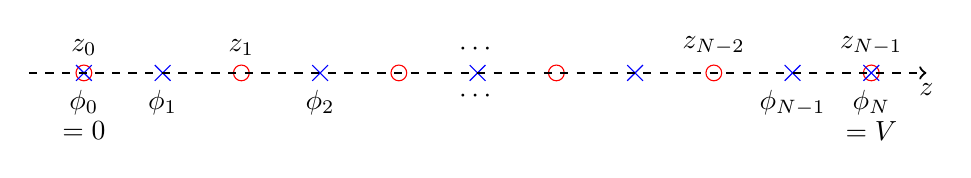
\begin{tikzpicture}
		\foreach \x in {1, 3, ..., 11}
		\draw[red] (\x, 0) circle (.1);

		\foreach \x in {1, 2, 4, ..., 10, 11}
			{
				\draw[xshift=\x cm, blue] (-.1, -.1) -- (.1, .1);
				\draw[xshift=\x cm, blue] (-.1, .1) -- (.1, -.1);
			}

		\draw (1, .1) node[above] {$z_0$};
		\draw (3, .1) node[above] {$z_1$};
		\draw (6, .1) node[above] {$\cdots$};
		\draw (9, .1) node[above] {$z_{N - 2}$};
		\draw (11, .1) node[above] {$z_{N - 1}$};

		\draw (1, -.1) node[below] {$\phi_0$};
		\draw (1, -.5) node[below] {$=0$};
		\draw (2, -.1) node[below] {$\phi_1$};
		\draw (4, -.1) node[below] {$\phi_2$};
		\draw (6, -.1) node[below] {$\cdots$};
		\draw (10, -.1) node[below] {$\phi_{N - 1}$};
		\draw (11, -.1) node[below] {$\phi_{N}$};
		\draw (11, -.5) node[below] {$= V$};

		\draw[->,thick,dashed] (.3, 0) -- (11.7, 0) node[below] {$z$};

	\end{tikzpicture}
	\caption{Discretization of the core potential $\phi_i = \phi(z_{i - 1/2})$;
	$\phi_0$ and $\phi_N$ are special and hold boundary conditions.}
	\label{fig:core_potential}
\end{figure}

The discretized core potential is defined at $z_0 = 0$, $z_{N-1} = h_s$
and the mid-points $z_{i + 1/2} = (z_i + z_{i + 1}) / 2$, see
fig.~\ref{fig:core_potential}:
\begin{equation}
	\begin{split}
		\phi_0 & = 0, \\
		\phi_1 & = \phi(z_{1/2}) = I \frac{r_c(z_0) \delta}{2}, \\
		\phi_2 & = \phi(z_{3/2}) = I \left[ \frac{r_c(z_0)}{2} +
			r_c(z_1) \right] \delta, \\
		\cdots \\
		\phi_N & = \phi(z_{N - 1}) = IR = V.
	\end{split}
\end{equation}
where the total resistance~$R$ is:
\begin{equation}
	R = \left[ \frac{r_c(z_0)}{2} + r_c(z_1) + \cdots + r_c(z_{N - 2}) +
	\frac{r_c(z_{N - 1})}{2} \right] \delta.
\end{equation}


% --------------------------------------------------------------------------------
%\section*{Interpolation between meshes}

% ================================================================================
\section{Device simulation algorithm}

The device simulation proceeds according to the following algorithm:

\begin{enumerate}
	\item \textbf{Initialization.} Read the mesh for the heat equations from the
	      external file; create the mesh for the Poisson equation; initialize the
	      finite-element solvers; initialize the Monte-Carlo solver; generate the
	      initial distribution of O-vacancies.

	\item Set bias voltage to zero: $V \gets 0$; set bias voltage sweep direction
	      to ``forward'': $\xi \gets +1$.

	\item \label{alg:main_compute_shape} \textbf{Main loop.} Compute the filament
	      shape.

	\item Compute the linear resistance $r_c(z)$; compute
	      the total current~$I$; compute the linear heat source density $I^2 r_c(z)$;
	      compute the Poisson equation boundary condition $\phi(0, z)$.

	\item Solve the heat equation for $T(r, z)$; solve the Poisson equation for
	      $\phi(r, z)$; interpolate to the Monte-Carlo grid to obtain $T(\vx_i)$
	      and $\phi(\vx_i)$.

	\item Estimate the duration $\langle \Delta t \rangle$ of a single Monte-Carlo
	      step. If it is larger than the minimum Monte-Carlo step duration
	      $\langle \Delta t \rangle_{\min} := \{ \mathsf{min\_step\_duration} \}$,
	      set time step: $\Delta t \gets \overline{\Delta t}_{\min}$, and go to
	      step \ref{alg:main_update_bias} (skip Monte-Carlo simulation).

	\item Run the Monte-Carlo simulation for $n := \{ \mathsf{steps\_per\_round} \}$
	      steps; compute the elapsed time $\Delta t$.

	\item \label{alg:main_update_bias} Update bias voltage:
	      $V \gets V + \xi s \Delta t$, where $s := \{ \mathsf{bias\_sweep\_rate} \}$
	      is the bias voltage sweep rate.

	\item Go to step \ref{alg:main_compute_shape}.
\end{enumerate}


\end{document}
